\chapter{Literature review}
\label{LR}

\section{Methods of Modelling Phages and Bacteria}
The most common way to model phages, bacteria, and resources populations and interactions is with Ordinary Differential Equations (ODEs) or Delay Differential Equations (DDE). 
DDEs are similar to ODEs, but DDEs incorporate time delays to account for processes that depend not only on the current state but also on past states, to incorporate behavior that has a delay, like latent infection time. 

One way to introduce a delay in an ODE model is to force populations to go through stages, causing a delay in other events. 
For example, in the paper \citet{gengUsingBacterialPopulation2024}, infected bacteria go through $M$ stages of infection, before lysing. 
By decreasing $\tau$ (the latent period) in the model proposed by \citet{gengUsingBacterialPopulation2024}, more infected bacteria go from infected state $i$ to infected state $i+1$ per timestep, causing the infected peak population count to peak earlier. 

The ODE method is simple to understand and easy to set up, but it can only capture large population dynamics.
Certain assumptions about the community interactions also have to be made, such as that everything is a probabilistic approach. 
Each model can be further developed, for example by adding temperature and pH dependence, bacteria releasing nutrients, or phage resistance. 

\subsection{Generalized Lotka-Volterra Model}
The Lotka-Volterra model, a first-order non-linear differential model, captures the dynamics between predators and prey.
Any population can be modelled as such:
\[ 
    \frac{d{B}_i}{dt} = {B}_i \left(\left(r_i + \sum_{j}^{N} \alpha_{ij}{B}_j \right) - m_i\right)
\]
where $r_i$ is reproduction rate, $\alpha_{ij}$ is the devour rate of $B_i$ on $B_j$. If $\alpha_{ij}$ is negative, then $B_i$ has a negative effect on $B_j$, otherwise $B_i$ has a positive effect on $B_j$. $m_i$ is the removal rate of $B_i$. 
The interactions can be seen in \Cref{fig:lotka_volterra_model}. 

It is possible to add phages into the system by 
 
\subsection{Generalized Consumer-Resource Model}
The generalized Consumer-Resource Model models the growth of a population and resource dynamics between a population of bacteria ${B}_i$ and a resource ${R}_i$. 
\begin{align}
    \frac{d{B}_i}{dt} &= r_i{B}_i \left(\sum_{\alpha} \Delta w_{i \alpha}C_{i \alpha}R_{\alpha}\right) - m_i {B}_i \label{eq:generalized_consumer_resource_model_1}\\
    \frac{dR_{\beta}}{dt} &= -\sum_i C_{i\beta}R_{\beta}{B_i} + \sum_{\alpha, i}D_{\beta\alpha}^{i}C_{i\alpha}R_{\beta}{B}_i \label{eq:generalized_consumer_resource_model_2}\\
    \Delta w_{i\alpha} &= \sum_{\beta}D_{\beta \alpha}^{i}w_{\beta} \nonumber
\end{align}
\Cref{eq:generalized_consumer_resource_model_1} describes the growth of population $B_i$ and \Cref{eq:generalized_consumer_resource_model_2} describes the resource dynamics and metabolism of resource $R_\beta$. 
Resource $R_\alpha$ can become resource $R_\beta$ at rate $R_{\beta \alpha}^{i}$. 
Bacteria $B_i$ reproduces at rate $r_i$ dependent on the concentration of resources $\sum_\alpha C_{i\alpha}$. 
Bacteria die out at rate $m_i$. 
For a visual, see \Cref{fig:consumer_resource_model}

\begin{figure}[h!]
    \centering
    \begin{subfigure}{0.49\linewidth}
        \centering
        \captionsetup{width=1\linewidth}
        \includegraphics[width=\linewidth]{Figures/lotka_volterra_model.png}
        \caption{
            Lotka-Volterra model.
        }
        \label{fig:lotka_volterra_model}
    \end{subfigure}
    \hfill
    \begin{subfigure}{0.49\linewidth}
        \centering
        \captionsetup{width=1\linewidth}
        \includegraphics[width=\linewidth]{Figures/consumer_resource_model.png}
        \caption{
            Consumer Resource model.
        }
        \label{fig:consumer_resource_model}
    \end{subfigure}
    \caption{Different models and how the bacterial entities interact with itself, one another, resources and the environment. All figures sourced from \citet{vandenbergEcologicalModellingApproaches2022}}. 
\end{figure}


\section{Phage Biology}
\subsection{What Are Phages?}
Phages are small bundles of proteins that contain viral DNA. 
Phages are made up of multiple parts built like LEGO to complete the task of infecting a bacterium. 
\Cref{fig:figures:phage_diagram} shows the body parts of a phage. 
The aim of the phage is to find a suitable bacterial host and infect the host with viral DNA. 
The DNA alters the host's metabolic pathways to its benefit and hijacks the cellular replication process to create new copies of the phage. 
Eventually, the cell lyses, releasing the newly created phages into the environment to infect more bacteria. 
\begin{figure}[h!]
    \centering
    \begin{subfigure}{0.25\linewidth}
        \centering
        \captionsetup{width=1\linewidth}
        \includegraphics[width=\linewidth]{Figures/phage_diagram.png}
        \caption{
            Phage body structure. 
            % (https://www.newyorker.com/tech/annals-of-technology/phage-killer-viral-dark-matter). 
        }
        \label{fig:figures:phage_diagram}
    \end{subfigure}
    \hfill
    \begin{subfigure}{0.3\linewidth}
        \centering
        \captionsetup{width=1\linewidth}
        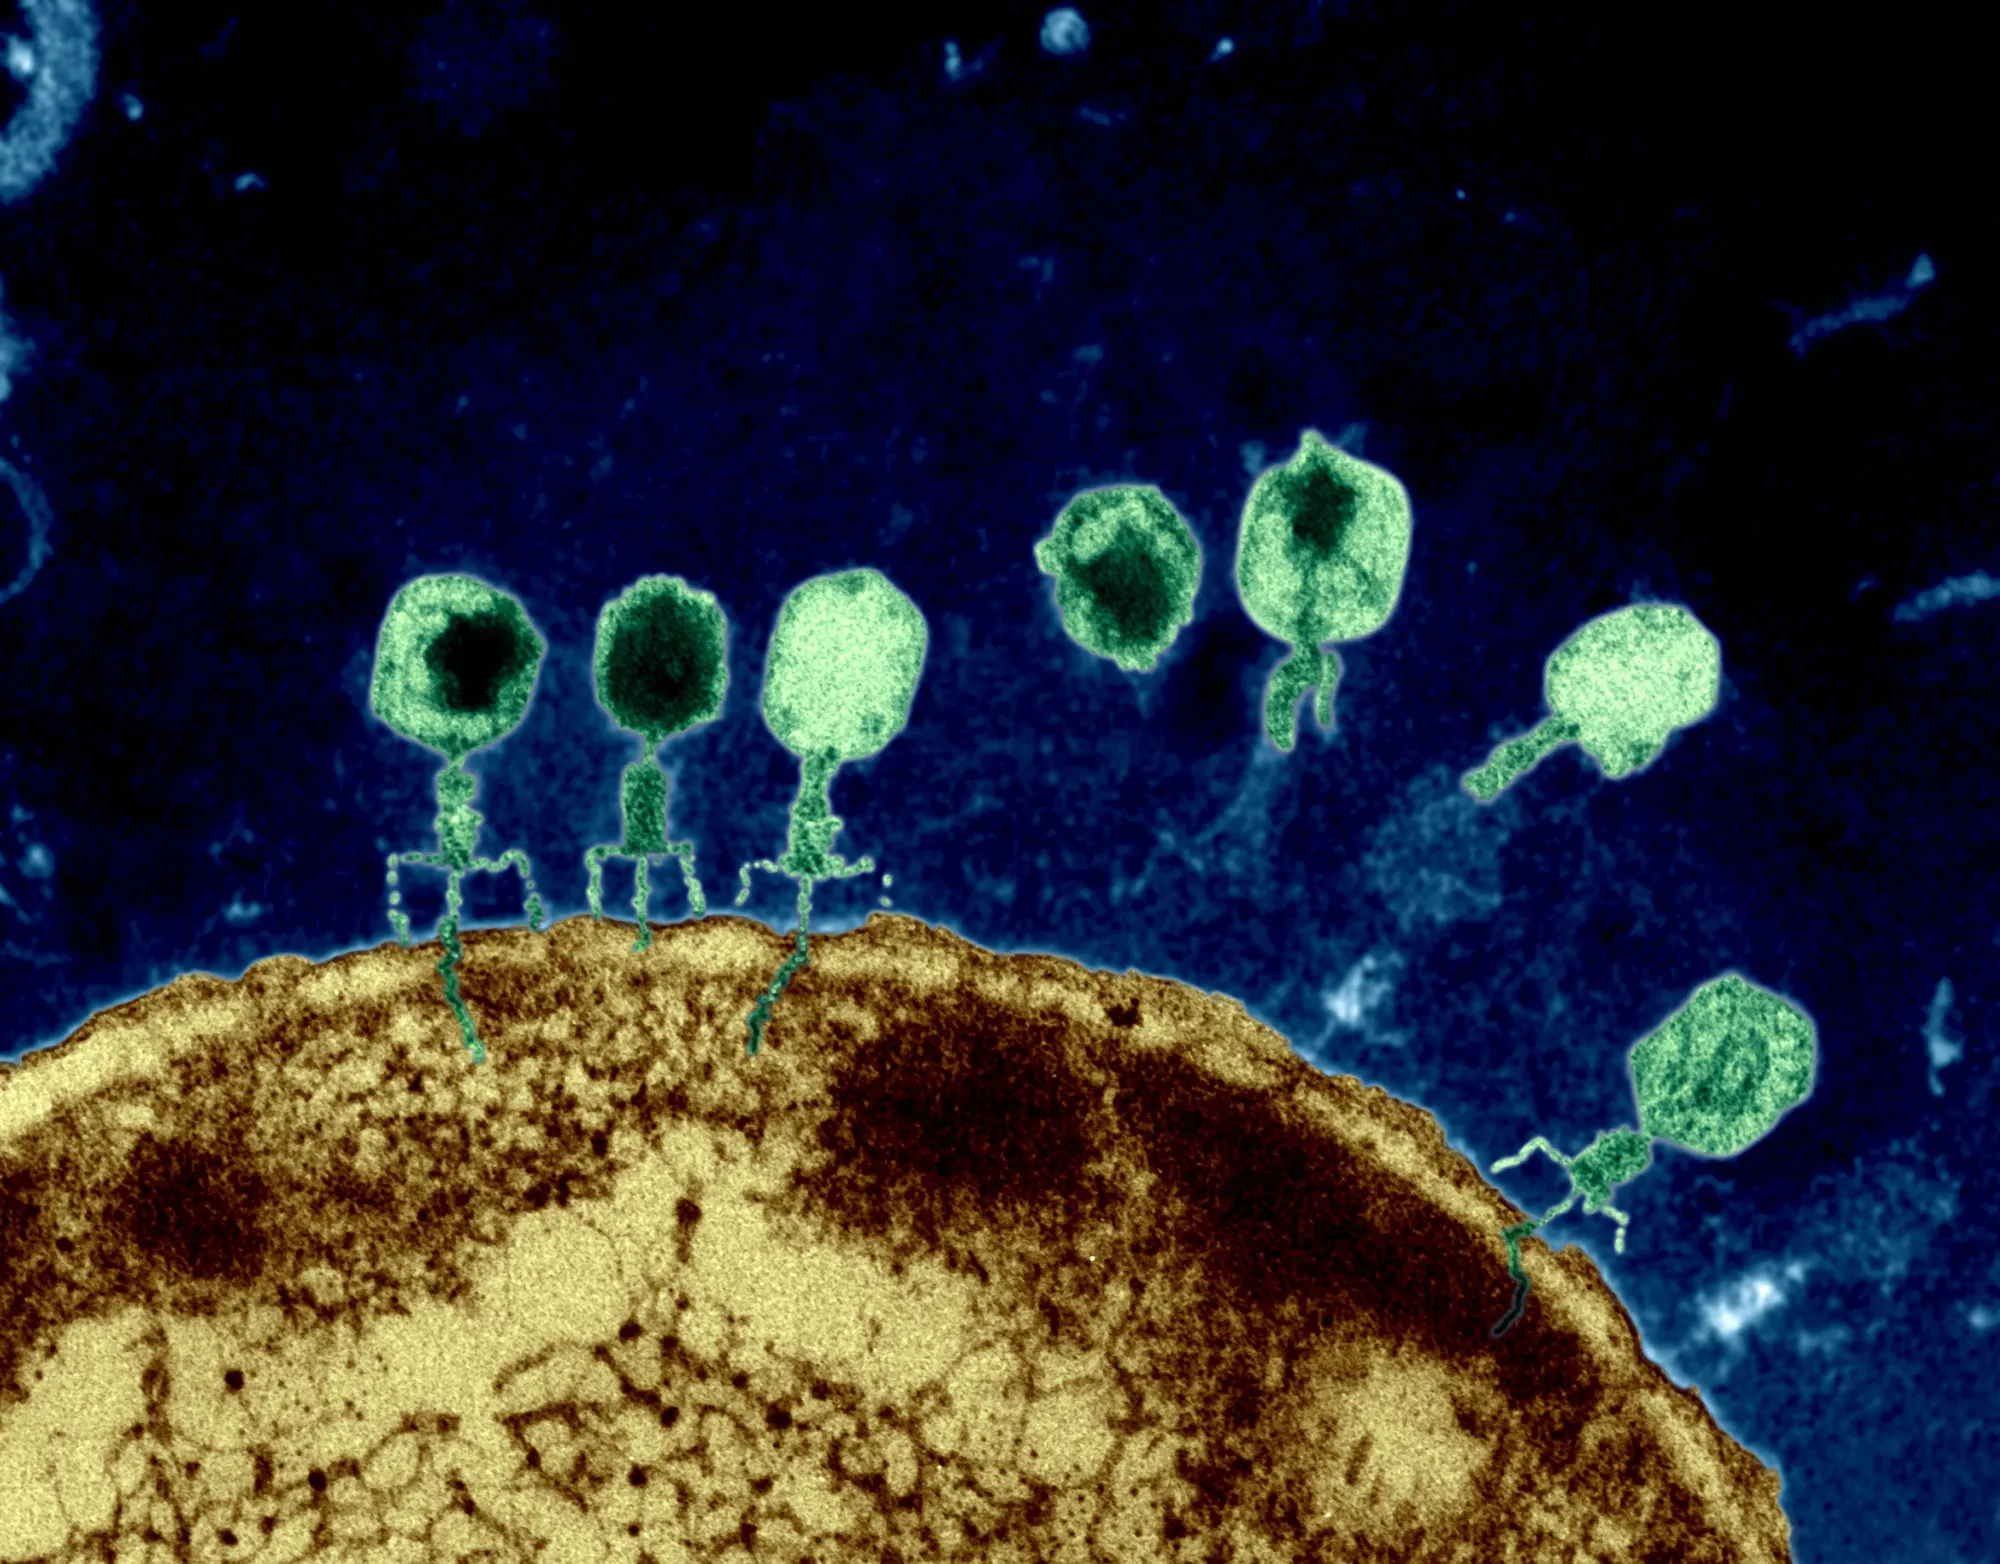
\includegraphics[width=\linewidth]{Figures/phage_real.png}
        \caption{
            Phages infecting an \textit{E. coli} bacteria. 
            % (https://www.newyorker.com/tech/annals-of-technology/phage-killer-viral-dark-matter). 
        }
        \label{fig:figures:phage_real}
    \end{subfigure}
    \hfill
    \begin{subfigure}{0.35\linewidth}
        \centering
        \captionsetup{width=1\linewidth}
        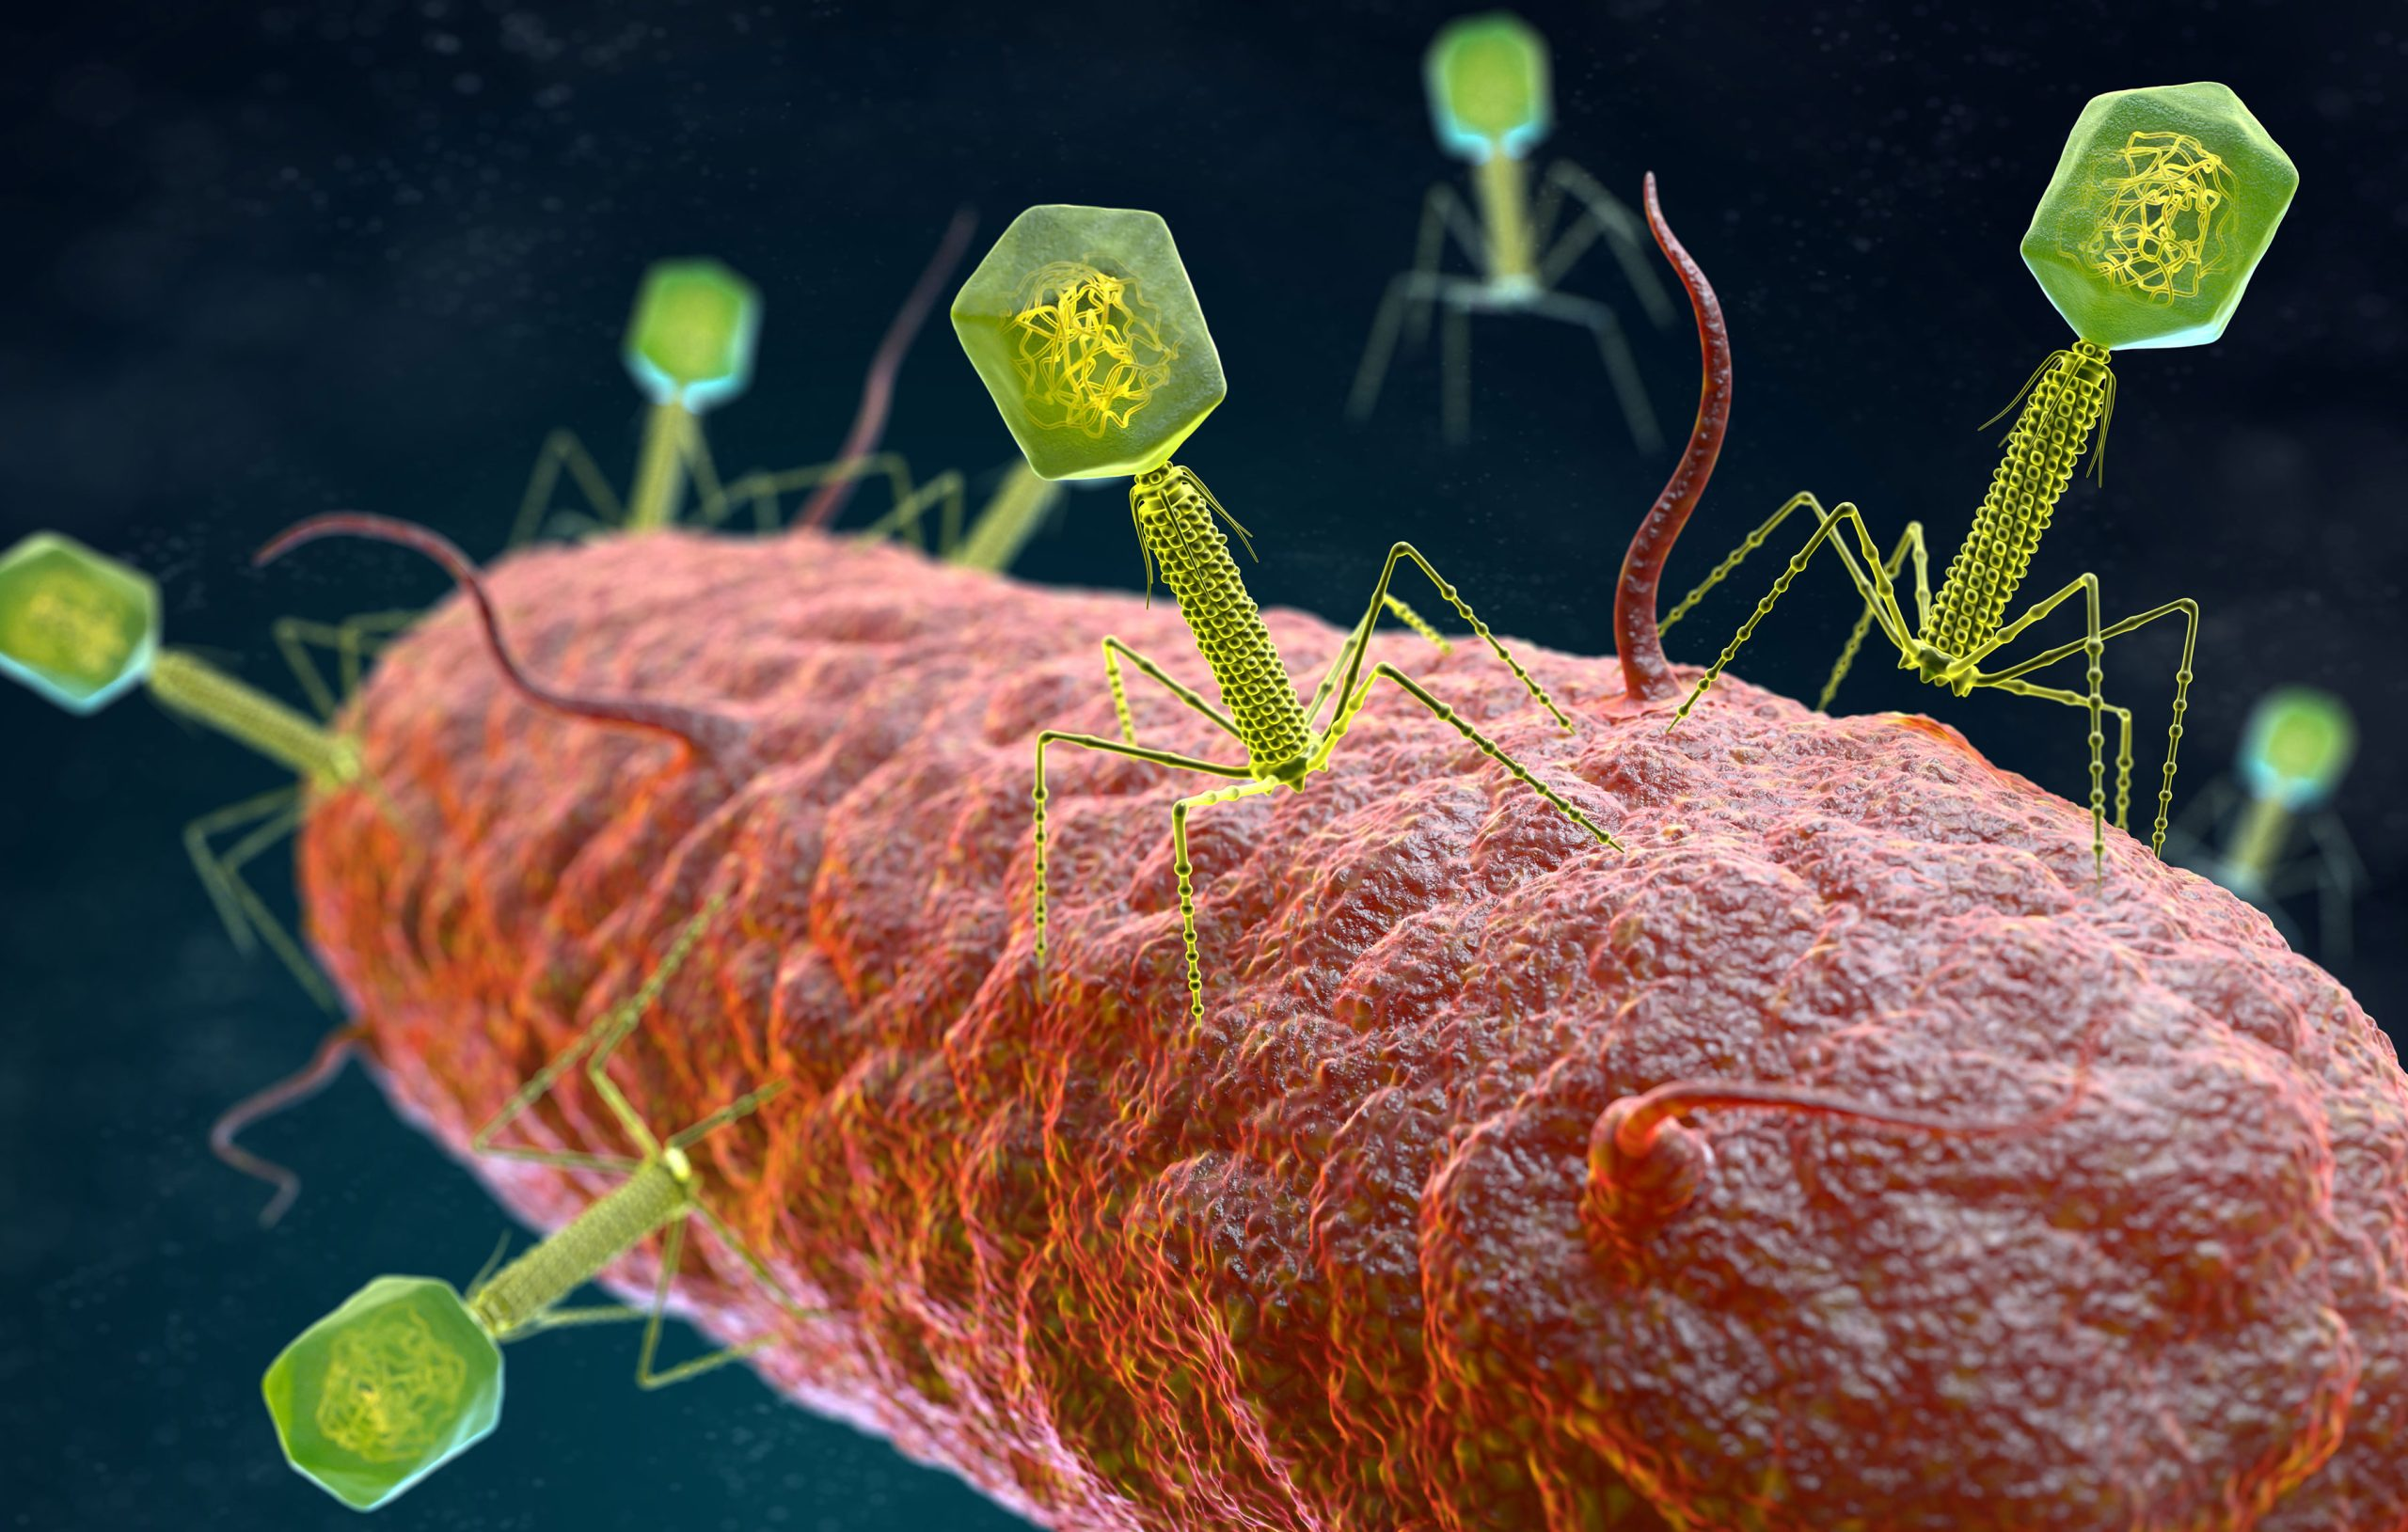
\includegraphics[width=\linewidth]{Figures/phage_impression.png}
        \caption{
            Artist representation of phages infecting a bacterium. 
            %(https://www.gettyimages.nl/detail/foto/bacteriophage-virus-attacking-a-bacterium-royalty-free-beeld/1179038792). 
        }
        \label{fig:figures:phage_impression}
    \end{subfigure}
    \caption{Parts of a phage, a real life picture of phages infecting an \textit{E. coli} bacterium, and an artist's impression of phages infecting a bacterium. }
\end{figure}

\subsection{How Does the Phage Cycle Work?}
There are 3 main parts to the phage-bacteria host cycle, the infection stage, the lysogenic cycle, and the lytic cycle. 
\Cref{fig:phage_life_cycle} shows a detailed overview of the phage cycle. 

In the infection stage, a phage attaches to the surface of a bacteria cell. 
The infection stage involves the phage searching for, detecting, and attaching to a bacterium, followed by DNA injection. 
Detection and attachment occur via phage receptor-binding proteins located at the tip of the phage tail that recognize specific receptors on the bacterial cell wall, triggering conformational changes that enable DNA injection. 
The success of this process depends on the specificity and density of both phage and bacterial receptors \cite{stoneUnderstandingExploitingPhage2019}. 
Once attached, the phage injects its DNA into the host cytoplasm, where it can replicate independently.
Once injected, the phage-cell pair can go into the lysogenic cycle or into the lytic cycle. 

The lysogenic cycle involves phage DNA integrating into the bacterial genome as a prophage, where it is replicated along with the host cell without causing immediate lysis.
The phage evades host defenses such as CBASS and CRISPR-Cas systems, which can start programmed cell death preventing phage replication or detect and degrade foreign DNA \cite{banhBacterialCGASSenses2023, levyCRISPRAdaptationBiases2015}. 
Programmed cell death helps recycle resources for other bacteria \cite{warwick-dugdaleHosthijackingPlanktonicPiracy2019}. 
Once integrated, the prophage can alter host fitness and provide resistance to other phages. 
During cell division, the prophage is copied into daughter cells but remains at risk of being excised by restriction enzymes \cite{sharpMolecularEvolutionBacteriophages1986}.
Under certain stress conditions, such as DNA damage or activation of the SOS response, the prophage can be induced to exit the genome and enter the lytic cycle \cite{waldorPhageRegulatoryCircuits2005, stoneUnderstandingExploitingPhage2019, fortierImportanceProphagesEvolution2013}.

The lytic cycle is the process where a phage infects a bacterium, hijacks its replication machinery to produce new phage components, assembles these parts, and ultimately lyses the host cell to release new phages. 
This involves hijacking the host's DNA replication to synthesize phage parts like the capsid, sheath, and tail \Cref{fig:figures:phage_diagram}. 
The phage does this by redirecting resources from internal cellular functions towards viral replication \cite{warwick-dugdaleHosthijackingPlanktonicPiracy2019}. 
The phage parts self-assemble via protein-protein and protein-nucleic acid interactions \cite{aksyukBacteriophageAssembly2011}. 
Phages induce bacterial lysis by producing holin proteins that disrupt the cell membrane, releasing the phages and resources \cite{wangHolinsProteinClocks2000}.

\section{Bacterial Defense Against Phages} 
\label{sec:literaturereview:bacterial_defense_against_phages}
There is a constant battle between phages and bacteria. 
The bacteria don't want to be killed by the phages, so they adapt defenses such as thickening of the cell wall or destroy the viral DNA. 

\subsection{Mutations in Bacterial DNA (Genetic (Co-)Evolution)}
As bacteria cells grow and divide, random point mutations can occur in the DNA. 
These mutations can affect phage defenses, like thickening the cell wall or removing a receptor, making it harder for the phages to detect and infect the cell. 
Mutations can be partially effective if full effectiveness requires multiple steps to achieve. 
Random mutations can also fail at making the bacteria more resistant to phages by increasing phage susceptibility or the mutation brings a cost to the bacteria cell by losing receptors on the cell wall \cite{lenskiTWOSTEPRESISTANCEESCHERICHIA1984}. 

\subsection{Horizontally Transferring DNA}
Bacteria can horizontally transfer DNA to other bacteria on contact. 
A donor cell can donate DNA fragments using a mechanism called a pilus. 
The pilus acts as a tunnel between the donor cell and the recipient cell so that DNA can be transferred from the donor cell to the receiver cell \cite{harbSsRNAPhagePenetration2020}. 

A phage can accidentally collect a piece of the host's DNA instead of its own DNA during assembly. 
The phage with the now dead hosts DNA can infect the next bacteria, injecting the new bacterium with the dead cell's DNA, horizontally transferring the DNA \cite{tamangHorizontalGeneTransfer2023, kasmanBacteriophages2025}. 
The transferred DNA can include natural phage defenses or significantly alter the genes and phenotype of the bacterium that future phages can't detect it anymore. 

\subsection{Phage Inactivation and Decoys}
Bacteria can further protect themselves by producing decoys that the phage will attach to instead of themselves. 
Freshly lysed bacteria may still have biomarkers that attract phages, leading phages to attach to non-viable cells where successful infection cannot occur.
Bacteria can also produce proteolytic enzymes that will damage the proteins found in a phage \cite{tanQuorumSensingDetermines2015}. 
Some bacteria can produce outer membrane vesicles that phages can absorb to, and later detach and float away with the phage \cite{rabinovitchBacterialDebrisEcological2003}. 
It is suspected that the impact of these vesicles acting as a sink is minor \cite{bullPhageBacterialDynamicsSpatial2018}. 

% \subsection{CRISPR-Cas Methods}
% CRISPR is a gene editing tool that cells can use to cut out specified/unwanted parts of a DNA strand. 
% Researchers are commonly using CRISPR to genetically engineer plants and animals to have specific features. 
% Strands of DNA can be selectively added or removed from a DNA strand to achieve a better, more desired DNA strand. 
% CRISPR defenses in the bacteria can detect the unwanted phage DNA and remove the DNA. 

\subsection{Phenotype Resistance}
Not all new phenotypes arise from genetic mutations. 
Resistance can result from phenotypic variation within a genetically identical population, allowing bacteria to express different resistance traits without altering their DNA.
\citet{guptaCombinatorialPhenotypicLandscape2025} found that some \textit{Bacteroides fragilis} bacteria were able to evade phage infection.  
The presence of combinatorial phenotypic states where differential expression of protective mechanisms created rare super-resistant cells capable of withstanding phage attack.
By acting together, these heterogeneously expressed anti-phage defense mechanisms created a phenotypic landscape where distinct protective combinations enabled the survival and re-growth of bacteria expressing these phenotypes without acquiring additional mutations. 

\subsection{Spatial Refuge/Biofilms} 
Usually bacteria and phages coexist in well mixed environments such as the ocean, however some environments offer natural structures for bacteria to hide behind. 
These structures can range from physical structure, like sediment in water to biochemical structures like biofilms, where the phages can't diffuse through the biofilm. 
In large enough quantities, bacteria and other microbial communities create biofilms, a layer of mucus containing various microbes. 
The thick mucus, microbes, and other spatial effects help protect the bacteria in the biofilm from external phages by making it hard for the phages to penetrate and diffuse through the mucus \cite{abedonPhageDelayEnhancing2017}. 
In the case of a lab experiment on an agar plate, bacteria protect one another by making it harder for the phages to diffuse through the system \cite{eriksenGrowingMicrocolonyCan2018}. 

Phage movement is passive, relying on diffusion through the environment or via pressure and temperature gradients \cite{lohrmannInfluenceBacterialSwimming2024}. 
Unlike phages, bacteria possess motility, allowing them to actively move through their environment increasing their chance of survival. 

\section{Phage Counter Defense Against Bacteria}
With some of the defenses that bacteria have developed, phages are always mutating to counter their defenses. 
If phages don't adapt to the ever-changing bacterial defenses, the phages will die out due to their inability to infect and multiply. 
It essentially becomes an arms race, seeing who can out-adapt the other. 
A delicate balance therefore needs to be achieved so that both the bacteria and the phages can coexist. 

\subsection{Genetic Mutations}
Mutations in viral DNA will affect how the phage body parts are designed and built. 
These mutations will affect external phage behavior such as how it detects a bacterium, as well as internal behavior such as evading detection and integrating with the cell's DNA. 
The changes will lead to changes in overall phage fitness, ie the ability for the phage to infect, replicate, and lyse bacteria. 

\subsection{Viral Recombination}
Multiple phages can infect a cell and replicate itself using the cells internal replication process. 
Each phage has its own building blocks. 
If the proteins that build the subparts of each phage have similar chemical properties, they can be swapped between phages \cite{aksyukBacteriophageAssembly2011}. 
This allows for biological diversity to spread throughout a phage population. 
Each phage body part can have unique characteristics such as better attachment rate, larger DNA storage capsule, or better probability of injection. 


\section{Phage Defense Against Phages}
Some phages can employ defenses against other phages from infecting the bacterial cell ensuring the host resources are all for itself. 
The act of preventing a secondary infection from a similar or closely related phage is called superinfection exclusion (SIE) \cite{patelAntiphageDefenceInhibition2024}. 
There are various methods of preventing further infections that are listed below. 

\subsection{Altering Cell Structure}
The prophage can alter the surface receptors of the bacteria, making it harder for other phages to detect the bacteria, reducing the chance of attachment and injection by other phages \cite{bucherPhageMachineSIEence2024}. 

\subsection{Protein Creation}
Other phages like the T4 phage can create proteins like the Spackle protein which inhibits the lysozyme activity used in the process of DNA injection by other phages \cite{bucherPhageMachineSIEence2024, kanamaruStructureFunctionT42020}. 
Some prophages can encode proteins that will interfere with the replication process of other phages. 
For example, the SieA protein encoded by phage P22 blocks infection from other phages \cite{leavittBacteriophageP22SieAmediated2024}. 

Tail Assembly Blocker (TAB) is an anti-phage defense mechanism encoded by a \textit{Pseudomonas aeruginosa} prophage. 
While TAB permits the invading phage to replicate its genome, it inhibits the assembly of the phage tail, thereby preventing the production of infectious virions. 
The prophage that encodes TAB is not affected by this inhibition, as it also expresses a protein that neutralizes TAB's blocking activity. 
Although the host cell still undergoes lysis, no infectious phages are released.

\subsection{Growth Curves Typically Seen in a Lab}
\label{sec:literaturereview:growth_curves_typically_seen_in_a_lab}

When choosing parameter values it is important to choose parameter values that could realistically be found in real life systems and be replicated in the lab. 
There are various features that a researcher will be looking for in growth curve produced in a lab.
A combination of these features results in an ideal growth curve that replicates real life bacterial growth. 

The idealized dynamics of bacterial populations undergoing phage infection have several phases. First, there is a clear exponential rise in bacteria growth, and can expect to grow 40-100x in the span of a few hours. 
At a certain point in time, the bacteria population start decreasing, almost as fast as they were growing. 

Phage populations also exhibit exponential growth, but with a delay in growth. 
There is initially no growth in phage population. 
After a set amount of time, the phage population will start to grow and peak a few hours after the bacteria population reached its peak. 
If there is no phage death or removal, the phage population will eventually reach a plateau when every bacteria has died. 

\Cref{fig:created:a_good_curve_linear} shows an example of a curve for a $1\times1\times1$ system that would typically be seen in a lab. 
\Cref{fig:created:a_good_curve_logarithmic} is the same plot but with a logarithmic y-axis. 
These specific plots exhibiting a clear growth, peak, delay, and death cycle. 

\begin{figure}[h!]
    \centering
    \begin{subfigure}{1\linewidth}
        \centering
        \captionsetup{width=1\linewidth}
        \includegraphics[width=\linewidth]{Plots/Created/a_good_curve_linear.png}
        \caption{
            An example linear y-axis for a curve that researchers aim to replicate. 
        }
        \label{fig:created:a_good_curve_linear}
    \end{subfigure}
    \hfill
    \begin{subfigure}{1\linewidth}
        \centering
        \captionsetup{width=1\linewidth}
        \includegraphics[width=\linewidth]{Plots/Created/a_good_curve_logarithmic.png}
        \caption{
            The equivalent logarithmic y-axis plot for a curve that researchers aim to replicate. 
        }
        \label{fig:created:a_good_curve_logarithmic}
    \end{subfigure}
    \caption{
        Growth population of a $1\times1\times1$ system. 
        The log plot allows to see behavior happening at values approaching and to plot data on a logarithmic scale. 
        The parameters used for this plot can be found in \Cref{tab:appendixE:a_good_curve}. 
    }
    \label{fig:created:a_good_curve}
\end{figure}

\section{Bacteria and Phages in the Lab}
Researchers around the world are running lab experiments to gain further knowledge of the interactions between phages and bacteria. 
The aim is to better understand how phages work and interact with bacteria at a molecular, host, and population level. 

\subsection{Running Experiments}
A researcher might run the experiment in a liquid medium containing water, carbon and nitrogen sources, and other chemicals such as anti-foaming or pH control chemicals. 
This liquid medium, often referred to as broth, allows for the cultivation of bacteria in a well-mixed environment, enabling researchers to monitor bacterial growth and phage infection dynamics over time. 
By adjusting parameters such as resource concentration, temperature, agitation speed, and pH, researchers can simulate different environmental conditions and observe their effects on phage-bacteria interactions. 

Samples can be taken at various time points to measure bacterial density, phage titer, and resource concentration, providing quantitative data for model validation and hypothesis testing. 
The researcher received an ODE-like curve of the bacteria density. 
Researchers can create a mathematical interpretation of the bacteria growth curve and run curve fitting algorithms to find the bacteria's growth rate. 
The phage parameters such as latent time and burst size can be found by analyzing the phage one-step growth curve \cite{gengUsingBacterialPopulation2024, mullaExtremeDiversityPhage2024}. 

\subsection{Chemostats}
Commonly used setups include liquids containing phages, bacteria, and resources in a chemostat and batch culture. 
Chemostats allow for continuous addition of resources and removal of waste, maintaining steady-state conditions ideal for studying long-term dynamics.
Bacteria density in clear liquid mediums can be measured optically using light. 
As the bacteria grow and die, the solution will get more cloudy. 
By shining a light through a vial with bacteria growth, the change in light refraction and intensity can be measured. 
A researcher might also be interested in using a mass spectrometer to measure the density of phages and resources at specific time points. 

\subsection{Petri Dishes}
Petri dishes are another commonly used way to grow bacterial colonies. 
Agar, a jelly-like substance derived from seaweed, is commonly used as a solid growth medium in petri dishes. 
Agar provides a stable surface for bacteria to grow on and form visible colonies. 
When phages are introduced, clear zones called plaques appear where phages have infected and lysed the bacteria, allowing for quantification and observation of phage activity. 
The phages can diffuse on the agar plate, infecting neighboring cells. 
Phage infection creates clear plaques (2-3 mm) where bacteria are absent. 
\Cref{fig:phage_petri_dish} shows an example of a bacteria lawn with phage plaques. 

\subsection{Measuring Growth}
Bacteria density in clear liquid mediums can be measured optically using light. 
As the bacteria grow and die, the solution will get more cloudy. 
By shining a light through a vial with bacteria growth, the change in light refraction and intensity can be measured. 
A researcher might also be interested in using a mass spectrometer to measure the density of phages and resources at specific time points. 

With petri dishes, it is harder to measure the bacterial growth. 
It might be possible to wash the bacteria off into a test tube with water to measure the optical density (OD), but the results are inconsistent. 
Even though using a special spectrophotometer allows consistent results, the results are dependent on the medium, the length of travel through the medium, bacteria size, and density. 
The device also has to be calibrated to ensure proper results, and results cant be compared across devices without calibration \cite{bealRobustEstimationBacterial2020}. 
Changing methods to using $\frac{\textit{cells}}{\textit{ml}}$ instead of OD can be used to directly compare results across experiments, labs, and bacteria colonies \cite{miraEstimatingMicrobialPopulation2022}. 

It might be possible to quantify the change in plaque size, either by hand or using an image analysis program, but the results might be inaccurate and sensitive to different lighting conditions. 

\begin{figure}[h!]
    \includegraphics[width=0.5\textwidth]{Figures/phage_petri_dish.jpeg}
    \centering
    \caption{
        Bacteria lawn, the dots on the petri dish show no bacteria growth due to the presence of phages. 
        Photo courtesy of S. Flickinger. 
    }
    \label{fig:phage_petri_dish}
\end{figure}
\subsection{Serial Transfer}
Serial transfer (ST) is a method employed by bacteriologist where after a set amount of time, the bacteriologist pipettes medium containing phages, bacteria, and resources out of a test tube and adds the old media into a new test tube with new media.
At this stage, the bacteriologist can add more bacteria or phages to the test tube. 
However, usually only resources are added during the transfer process.
Researchers can optically measure the bacteria density using an optical density machine or employ a mass spectrometer to determine the phage concentration at set time points during the experiment. 
As the bacteria grow, they consume the resources found in the medium.
The resources will eventually run out, and the bacteria die out due to a lack of resources.
By introducing new resources at set time intervals, the bacteria can regrow and exhibit a semi-stationary behavior.

\subsection{Growth Curves Typically Seen in a Lab}
\label{sec:literaturereview:growth_curves_typically_seen_in_a_lab}

When choosing parameter values it is important to choose parameter values that could realistically be found in real life systems and be replicated in the lab. 
There are various features that a researcher will be looking for in growth curve produced in a lab.
A combination of these features results in an ideal growth curve that replicates real life bacterial growth. 

The idealized dynamics of bacterial populations undergoing phage infection have several phases. First, there is a clear exponential rise in bacteria growth, and can expect to grow 40-100x in the span of a few hours. 
At a certain point in time, the bacteria population start decreasing, almost as fast as they were growing. 

Phage populations also exhibit exponential growth, but with a delay in growth. 
There is initially no growth in phage population. 
After a set amount of time, the phage population will start to grow and peak a few hours after the bacteria population reached its peak. 
If there is no phage death or removal, the phage population will eventually reach a plateau when every bacteria has died. 

\Cref{fig:created:a_good_curve_linear} shows an example of a curve for a $1\times1\times1$ system that would typically be seen in a lab. 
\Cref{fig:created:a_good_curve_logarithmic} is the same plot but with a logarithmic y-axis. 
These specific plots exhibiting a clear growth, peak, delay, and death cycle. 

\begin{figure}[h!]
    \centering
    \begin{subfigure}{1\linewidth}
        \centering
        \captionsetup{width=1\linewidth}
        \includegraphics[width=\linewidth]{Plots/Created/a_good_curve_linear.png}
        \caption{
            An example linear y-axis for a curve that researchers aim to replicate. 
        }
        \label{fig:created:a_good_curve_linear}
    \end{subfigure}
    \hfill
    \begin{subfigure}{1\linewidth}
        \centering
        \captionsetup{width=1\linewidth}
        \includegraphics[width=\linewidth]{Plots/Created/a_good_curve_logarithmic.png}
        \caption{
            The equivalent logarithmic y-axis plot for a curve that researchers aim to replicate. 
        }
        \label{fig:created:a_good_curve_logarithmic}
    \end{subfigure}
    \caption{
        Growth population of a $1\times1\times1$ system. 
        The log plot allows to see behavior happening at values approaching and to plot data on a logarithmic scale. 
        The parameters used for this plot can be found in \Cref{tab:appendixE:a_good_curve}. 
    }
    \label{fig:created:a_good_curve}
\end{figure}

\section{Software Mathematically Modelling Phages, Bacteria, and Resources}
Some software programs modelling phage-bacteria-resource interactions already exists. 
\subsection{Cocktail}
\citet{nilssonCocktailComputerProgram2022} developed Cocktail to model phage-bacteria-resource kinetics in a chemostat. 
The model assumes there is one bacteria strain that can be infected by phage A and phage B, and by both phages at the same time, phage AB. 
The model models bacterial resistance to phage A, B, and AB. 
The user can control the parameter values such as resistance rate to A, B, and AB, resource concentration and outflow, and phage adsorption rate. 
The user can also control model settings, such as if the model is deterministic or stochastic, and the step size \cite{nilssonCocktailComputerProgram2022}. 
Four sample output plots are shown in \Cref{fig:sourced:cocktail_plot}. 

\subsection{PhageDyn}
PhageDyn is a Java applet that models phage dynamics in multi-reactor industrial wastewater treatment plant models. 
PhageDyn interacts with existing GPS-X \cite{AdvancedWastewaterModelling} files to incorporate phage dynamics into models of industrial wastewater treatment plants \cite{krysiak-baltynSimulationPhageDynamics2017}. 
\citet{krysiak-baltynSimulationPhageDynamics2017} developed PhageDyn to determine how phages can reduce foaming caused by bacteria in wastewater treatment plants, another real life application of phages \cite{heardEffectFilamentousBacteria2008}. 
PhageDyn does not simulate phage dynamics on its own but rather manipulates existing files in GPS-X in order to incorporate phage dynamics in wastewater treatment plant models. 
\Cref{fig:sourced:phagedyn_plot} shows the output that PhageDyn provides. 

\subsection{Cocktail and PhageDyn Limitations}
\label{sec:literature:cocktail_and_phagedyn_limitations}
There are limitations to Cocktail and PhageDyn. 
Cocktail can model up to a $2\times 1 \times 1$ system, and is designed to model a chemostat. 
Chemostats receive a constant influx of new resources and a constant removal of medium from the chemostat. 
Cocktail's model can not be easily adapted to other models. 
The ODE model accepts inputs from a hardcoded GUI frontend. 
So any changes to the frontend or to the ODE model will require changes to the ODE model and the frontend to accept the new inputs and outputs. 
The code for Cocktail is open source, so adding new buttons and changing the model should not pose a significant challenge, but still an undertaking. 

PhageDyn works with GPS-X, a very niche wastewater treatment modelling software. 
PhageDyn is programmed for a very specific task with no flexibility in changing the model or inputs. 
PhageDyn assumes biomass, instead of individual bacteria populations. 
However, PhageDyn is no longer available for download.

\begin{figure}
    \centering
    \begin{subfigure}{0.49\linewidth}
        \centering
        \captionsetup{width=1\linewidth}
        \includegraphics[width=\linewidth]{Plots/Sourced/cocktail_plot.png}
        \caption{
            Figure A) \textit{E. coli} infected with phage T4 in a chemostat exhibiting an oscillating growth behavior, following the model of \citet{bohannanEffectResourceEnrichment1997}. 
            Figure B) Oscillations of bacteria and phages can exist at higher titers, dependent on low resource concentration, following the model of \citet{lenskiDynamicsInteractionsBacteria1988}. 
            Figure C) As the concentration of resources change, this results in increasing oscillations, but not going extinct. 
            Figure D) A system modelling the interactions with phage A and B. 
        }
        \label{fig:sourced:cocktail_plot}
    \end{subfigure}
    \hfill
    \begin{subfigure}{0.49\linewidth}
        \centering
        \captionsetup{width=1\linewidth}
        \includegraphics[width=\linewidth]{Plots/Sourced/phagedyn_plot.png}
        \caption{
            \textcolor[HTML]{551A8C}{\textbf{Purple}} is heterotrophic biomass, 
            \textcolor[HTML]{4580B4}{\textbf{Blue}} is foaming biomass, 
            \textcolor[HTML]{FF0000}{\textbf{Red}} is phages, 
            \textcolor[HTML]{01E6EE}{\textbf{Light Blue}} is total suspended solids. 
            Figure A) Biomass concentration immediately post phage dosing. 
            Figure B) Biomass concentration with low phage concentration and maintain low concentration post spike in population count. 
            Figure C) Biomass concentration when phages are extinct. 
            Figure D) Biomass concentration with a less virulent and low adsorption rate phage, co-existence with biomass reached. 
            A change in phage concentration shows a decrease in heterotrophic and foaming biomass \cite{krysiak-baltynSimulationPhageDynamics2017}. 
        }
        \label{fig:sourced:phagedyn_plot}
    \end{subfigure}
    \caption{Example output from Cocktail and PhageDyn respectively. For PhageDyn, concentration of heterotrophic biomass in an aerobic plug flow across four situations.
        See \citet{nilssonCocktailComputerProgram2022} and \citet{krysiak-baltynSimulationPhageDynamics2017} for more information on parameter values and supplementary resources. 
    }
    \label{fig:sourced:cocktail_and_phagedyn}
\end{figure}

\section{The Golding Model}
\label{sec:golding_model}
The default model that will be used in this thesis, the “Golding model“, sourced from \citet{gengUsingBacterialPopulation2024}, describes the interactions between resources, uninfected bacteria, infected bacteria, and phages. 

\subsection{The Original Golding Model}
The model describes three biological processes, cell consumption of resources and growing, phage/cell encounters and infection, and cell lysis. 
The cell growth process is described by $g(R, v, K)$, the instantaneous growth rate dependent on the Monod equation, where $v$ is the maximal growth rate of the bacteria population and $K$ is the Monod constant. 
Bacteria consume a resource with rate $e$. 

Once infected by a phage, the bacteria goes from $U$ to $I_1$. 
The bacteria goes through $M$ stages of infection $I_1, \dots, I_M$ before lysing, 
The bacteria goes from state $I_k$ to state $I_{k+1}$ with equal transition rate $\frac{M}{\tau}$. 
The infection rate of a cell is $r$. 
After a bacteria lyses after stage $I_M$, $\beta$ phages are released, the burst size of the phage. 

\begin{eqfloat}[ht!]
    \begin{align}
        \frac{dR}{dt} &= -e \cdot g(R, v, K)\cdot (U + \sum_{k=1}^{M} I_k)\\
        \frac{dU}{dt} &= g(R, v, K)\cdot U - r\cdot U \cdot P\\
        \frac{dI_1}{dt} &= r\cdot U \cdot P - \frac{M}{\tau}\cdot I_1\\
        \frac{dI_k}{dt} &= \frac{M}{\tau}(I_{k-1}-I_k) \text{ for } k=2, \dots, M \\
        \frac{dP}{dt} &= \beta \cdot\frac{M}{\tau} \cdot I_M - r\cdot(U + \sum_{k=1}^{M} I_k)\cdot P \\
        g(R, v, K) &= \frac{v\cdot R}{R + K}
        \label{eq:golding_model}
    \end{align}
    \caption{
        The Golding model sourced from \citet{gengUsingBacterialPopulation2024}. 
        The text in \textcolor{red}{red} has been added to the model, adding (the wash-in) fresh resources ($\omega^i$) and the removal (wash-out) of entities ($\omega^o$). 
        The washin is not dependent on the current resource population, as it is a constant rate being added. 
        By default these values are 0.
        A summary of the parameters can be found at \Cref{tab:appendixA:parameter_table_simple_golding_model}. 
    }
\end{eqfloat}

\subsection{The Adapted Golding Model}
\label{sec:adapted_golding_model}
The original Golding model is specifically designed for a $1\times 1 \times 1$ system. 
In order to adapt this model to fit an $p \times b \times r$ model, the model needs to be slightly adapted. 
There are other changes that can be made to the model, for example by adding a washin rate $\omega^{i}$, where resources are constantly being introduced, and a washout rate $\omega^{o}$ where all entities are washed out at a constant rate. 
These changes are highlighted in \Cref{eq:adapted_golding_model} in \textcolor{red}{red}. 

The adapted model accounts for the interactions of multiple phages, bacteria, and resources, and assumes the interactions occur independently of one another. 

\begin{eqfloat}
    \begin{align}
        \frac{dR_r}{dt} &= -\sum_{b \in B} e_{b r} \cdot g(R_r, v_{b r}, K_{b r})\cdot (U_b + \sum_{k=1}^{M} I_{b_k}) \mathcolor{red}{+ w^i -w^o \cdot R_r}\\
        \frac{dU_b}{dt} &= U_b \cdot \sum_{r \in R} g(R_r, v_{b r}, K_{b r}) - U_b \cdot \sum_{p \in P} r_{p b} \cdot P_p -\mathcolor{red}{-w^o \cdot U_b}\\
        \frac{dI_{b_1}}{dt} &= U_b \cdot \sum_{p \in P}r_{p b} \cdot P_p - \frac{M}{\tau_b}\cdot I_{b_1} \mathcolor{red}{-w^o \cdot I_{b_1}}\\
        \frac{dI_{b_k}}{dt} &= \frac{M}{\tau_b}(I_{b_{k-1}}-I_{b_k}) \mathcolor{red}{-w^o \cdot I_{b_k}}\text{ for } k=2, \dots, M \\
        \frac{dP_p}{dt} &= \sum_{b\in B}\beta_{p b}\cdot\frac{M}{\tau_b} \cdot I_{b_M} - r_{p b}\cdot(U_b + \sum_{k=1}^{M} I_{b_k})\cdot P_p \mathcolor{red}{-w^o \cdot P_p}\\
        g(R_r, v_{b r}, K_{b r}) &= \frac{v_{b r} \cdot R_r}{R_r + K_{b r}}
        \label{eq:adapted_golding_model}
    \end{align} 
    \caption{
        The adapted Golding model. 
        The probability of phage $p$ infecting bacteria $b$ is $r_{p b}$ is not to be confused with the resource concentration $R_r$. 
        The interactions are a sum of all interactions due to all interactions taking place at the same time. 
    }
\end{eqfloat}